
\documentclass[10pt,a4paper]{article}
\usepackage[a4paper,margin=13mm,top=11mm,bottom=12mm]{geometry}
\usepackage{fontspec}
\usepackage{xcolor}
\usepackage{graphicx}
\usepackage{tabularx}
\usepackage{array}
\usepackage{fancyhdr}
\defaultfontfeatures{Ligatures=TeX}
\IfFontExistsTF{Noto Sans CJK SC}{\setmainfont{Noto Sans CJK SC}\setsansfont{Noto Sans CJK SC}}{\setmainfont{DejaVu Sans}\setsansfont{DejaVu Sans}}
\definecolor{BOBlue}{HTML}{0055A4}
\definecolor{BOBright}{HTML}{3273F6}
\definecolor{BONavy}{HTML}{051C2C}
\definecolor{BOMuted}{HTML}{6F7F8F}
\definecolor{BOLine}{HTML}{DCE3EA}
\definecolor{BOLight}{HTML}{F4F8FC}
\setlength{\parindent}{0pt}
\setlength{\parskip}{3.2pt}
\setlength{\tabcolsep}{4pt}
\renewcommand{\arraystretch}{1.15}
\hyphenpenalty=10000
\exhyphenpenalty=10000
\tolerance=4000
\emergencystretch=2em
\sloppy
\pagestyle{fancy}
\fancyhf{}
\renewcommand{\headrulewidth}{0pt}
\renewcommand{\footrulewidth}{0pt}
\fancyhead[L]{\scriptsize\color{BOMuted} BLUEOCEAN | CONFIDENTIAL}
\fancyfoot[L]{\scriptsize\color{BOMuted} BlueOcean | Confidential}
\fancyfoot[R]{\scriptsize\color{BOMuted} \thepage}
\newcolumntype{Y}{>{\raggedright\arraybackslash}X}

\begin{document}
\raggedright
\thispagestyle{empty}

\includegraphics[width=\paperwidth,height=\paperheight]{assets/cover-background.png}\par
\vspace*{10mm}
{\textcolor{BOBlue}{\scriptsize\bfseries BLUEOCEAN\\DEEP RESEARCH REPORT}}\par\vspace{8mm}
{\fontsize{24}{27}\selectfont\color{BONavy} Strategic Assessment of the Agricultural Sector: Navigating Disruption and Unlocking Growth}\par\vspace{6mm}
{\small\color{BOMuted} A BlueOcean Research Report for Senior Executives and Policymakers}\clearpage

{\textcolor{BOBlue}{\scriptsize\bfseries KEY HIGHLIGHTS}}\par\vspace{-1pt}
{\Large\sffamily\bfseries\color{BONavy} The report opens with decision-relevant conclusions}\par\vspace{4pt}
\vspace{2pt}{\color{BOBright}\rule{\linewidth}{1pt}}\vspace{5pt}
\begin{tabularx}{\linewidth}{p{12mm}Y}
\textcolor{BOBlue}{\bfseries 01} & {\small The global agricultural sector is at a critical inflection point, facing unprecedented disruption from climate change, technological innovation, and shifting trade policies.} \\[5pt]
\textcolor{BOBlue}{\bfseries 02} & {\small This strategic assessment identifies that while demand for food continues to outpace sustainable supply expansion, digital and precision agriculture offer the highest return on investment for productivity gains.} \\[5pt]
\textcolor{BOBlue}{\bfseries 03} & {\small However, water scarcity and soil degradation pose the most critical long-term risks, requiring immediate attention.} \\[5pt]
\textcolor{BOBlue}{\bfseries 04} & {\small Regulatory shifts in Europe and evolving trade tensions are reshaping competitive landscapes, while alternative proteins and vertical farming present high-growth adjacencies.} \\[5pt]
\textcolor{BOBlue}{\bfseries 05} & {\small Carbon markets create new revenue streams but depend on robust verification standards.} \\[5pt]
\textcolor{BOBlue}{\bfseries 06} & {\small The report outlines seven strategic priorities for the next 3-5 years, emphasizing climate-smart practices, technology adoption, and risk mitigation to secure a resilient and profitable agricultural future.} \\[5pt]
\end{tabularx}
\clearpage

{\textcolor{BOBlue}{\scriptsize\bfseries CONTENTS}}\par\vspace{-1pt}
{\Large\sffamily\bfseries\color{BONavy} Contents}\par\vspace{4pt}
\vspace{2pt}{\color{BOBright}\rule{\linewidth}{1pt}}\vspace{5pt}
\begin{tabularx}{\linewidth}{p{10mm}Y}
\textcolor{BOBlue}{\bfseries 1} & Agriculture faces unprecedented disruption from climate change and technology \\[4pt]
\textcolor{BOBlue}{\bfseries 2} & Global demand growth is outpacing sustainable supply expansion \\[4pt]
\textcolor{BOBlue}{\bfseries 3} & Digital and precision agriculture offer the highest ROI for productivity gains \\[4pt]
\textcolor{BOBlue}{\bfseries 4} & Regulatory shifts in Europe and trade tensions reshape competitive landscape \\[4pt]
\textcolor{BOBlue}{\bfseries 5} & Water and soil health are the most critical long-term risks \\[4pt]
\textcolor{BOBlue}{\bfseries 6} & Alternative proteins and vertical farming represent high-growth adjacencies \\[4pt]
\textcolor{BOBlue}{\bfseries 7} & Carbon markets create new revenue streams but require verification standards \\[4pt]
\textcolor{BOBlue}{\bfseries 8} & Strategic priorities for the next 3-5 years require decisive action \\[4pt]
\end{tabularx}
\clearpage

{\textcolor{BOBlue}{\scriptsize\bfseries DISCLAIMER}}\par\vspace{-1pt}
{\Large\sffamily\bfseries\color{BONavy} Disclaimer}\par\vspace{4pt}
\vspace{2pt}{\color{BOBright}\rule{\linewidth}{1pt}}\vspace{5pt}
{\small This document is for management research and strategy discussion only.}\par
\vspace{6pt}{\scriptsize\color{BOMuted} This report was informed by public research and data from: Ipcc, Fao, Wri, Bloomberg, Marketsandmarkets, Grandviewresearch, Ecosystemmarketplace, Europa.}\vspace{6pt}
{\scriptsize\color{BOMuted} Full source backup is archived in the backup folder.}\clearpage

\clearpage
{\textcolor{BOBlue}{\scriptsize\bfseries CHAPTER 1}}\par\vspace{-1pt}
{\Large\sffamily\bfseries\color{BONavy} Agriculture faces unprecedented disruption from climate change and technology}\par\vspace{4pt}
\begin{minipage}[t]{0.58\linewidth}
{\small Climate change is fundamentally altering agricultural productivity, with rising temperatures, shifting precipitation patterns, and increased frequency of extreme weather events reducing crop yields globally. The Intergovernmental Panel on Climate Change projects that without adaptation, global crop yields could decline by up to 25\% by 2050, threatening food security and supply chain stability. This disruption is not uniform; tropical and subtropical regions face the most severe impacts, while temperate zones may experience some benefits from longer growing seasons, creating a complex mosaic of winners and losers.}

{\small Simultaneously, technological innovation is accelerating at an unprecedented pace. Precision agriculture, artificial intelligence, and biotechnology are transforming farming practices, enabling higher yields with fewer inputs. The global precision agriculture market is projected to reach \$12.8 billion by 2025, driven by adoption of GPS-guided tractors, drone monitoring, and variable rate irrigation. These technologies offer a pathway to resilience, but their high upfront costs and digital divide risks could exacerbate inequalities between large commercial farms and smallholders.}
\end{minipage}\hfill
\begin{minipage}[t]{0.36\linewidth}

\includegraphics[width=58mm,height=45mm,keepaspectratio]{assets/image-1.png}
\end{minipage}
\vspace{3pt}\noindent\fcolorbox{BOLine}{BOLight}{\parbox{0.965\linewidth}{\small \textbf{So what:} \textbullet\ Validate assumptions with source backup.}}\vspace{4pt}
{\small {\small The convergence of climate stress and technological opportunity creates a strategic imperative for agribusiness leaders and policymakers. Investments in climate-smart agriculture and digital infrastructure are no longer optional but essential for long-term competitiveness. Companies that fail to adapt risk being marginalized, while early adopters can capture significant market share and operational efficiencies.}}
\vspace{4pt}{\textcolor{BOBlue}{\scriptsize\bfseries ANALYTIC CHECKLIST}}\par\begin{tabularx}{\linewidth}{p{42mm}Y}
Market signal & Structural demand \\ 
Capability & Scale and proof \\ 
Execution & Risks and actions \\ 
\end{tabularx}

\clearpage
{\textcolor{BOBlue}{\scriptsize\bfseries CHAPTER 2}}\par\vspace{-1pt}
{\Large\sffamily\bfseries\color{BONavy} Global demand growth is outpacing sustainable supply expansion}\par\vspace{4pt}
\begin{minipage}[t]{0.58\linewidth}
{\small Global food demand is projected to increase by 60\% by 2050, driven by population growth and rising incomes in developing economies, particularly in Asia and Africa. This demand surge is straining natural resources, with agricultural land expansion already limited by urbanization, deforestation regulations, and land degradation. The Food and Agriculture Organization estimates that only 10\% of additional food production can come from land expansion, necessitating a 90\% increase in productivity on existing farmland.}

{\small Sustainable supply expansion faces multiple bottlenecks. Water scarcity affects over 40\% of the world's agricultural areas, with groundwater depletion accelerating in key production zones like the Indo-Gangetic Plain and California's Central Valley. Soil degradation, including erosion and nutrient depletion, reduces productivity on one-third of global farmland. These constraints are compounded by labor shortages, as rural populations age and younger generations migrate to cities, leaving a shrinking workforce to manage increasingly complex operations.}
\end{minipage}\hfill
\begin{minipage}[t]{0.36\linewidth}

\includegraphics[width=58mm,height=45mm,keepaspectratio]{assets/image-2.png}
\end{minipage}
\vspace{3pt}\noindent\fcolorbox{BOLine}{BOLight}{\parbox{0.965\linewidth}{\small \textbf{So what:} \textbullet\ Validate assumptions with source backup.}}\vspace{4pt}
{\small {\small The gap between demand and sustainable supply presents both a risk and an opportunity. Agribusinesses that invest in yield-enhancing technologies, water-efficient irrigation, and soil health programs can capture premium markets and build long-term resilience. Policymakers must prioritize research and development, infrastructure investment, and incentives for sustainable practices to close the supply gap without environmental collapse.}}
\vspace{4pt}{\textcolor{BOBlue}{\scriptsize\bfseries ANALYTIC CHECKLIST}}\par\begin{tabularx}{\linewidth}{p{42mm}Y}
Use case & Priority logic \\ 
Near term & Clear proof path \\ 
Longer term & Monitor options \\ 
\end{tabularx}

\clearpage
{\textcolor{BOBlue}{\scriptsize\bfseries CHAPTER 3}}\par\vspace{-1pt}
{\Large\sffamily\bfseries\color{BONavy} Digital and precision agriculture offer the highest ROI for productivity gains}\par\vspace{4pt}
\begin{minipage}[t]{0.58\linewidth}
{\small Digital agriculture technologies, including IoT sensors, satellite imagery, and farm management software, enable real-time monitoring and data-driven decision-making. Early adopters report yield increases of 10-20\% and input cost reductions of 15-30\%, delivering strong returns on investment. Precision agriculture tools such as variable rate fertilization and automated irrigation optimize resource use, reducing waste and environmental impact while boosting profitability.}

{\small The adoption of digital twins—virtual replicas of physical farms—is emerging as a game-changer for large-scale operations. These models simulate crop growth, weather scenarios, and resource allocation, allowing farmers to test strategies before implementation. By 2025, digital twin technology is expected to be used on over 5 million hectares globally, primarily in North America and Europe, with potential to reduce water usage by 20\% and fertilizer application by 15\%.}
\end{minipage}\hfill
\begin{minipage}[t]{0.36\linewidth}

\includegraphics[width=58mm,height=45mm,keepaspectratio]{assets/image-3.png}
\end{minipage}
\vspace{3pt}\noindent\fcolorbox{BOLine}{BOLight}{\parbox{0.965\linewidth}{\small \textbf{So what:} \textbullet\ Validate assumptions with source backup.}}\vspace{4pt}
{\small {\small However, the digital divide remains a significant barrier. Smallholder farmers, who produce over 70\% of the world's food, often lack access to affordable technology, connectivity, and training. Bridging this gap requires public-private partnerships, subsidized technology packages, and extension services tailored to local contexts. Agribusinesses that develop inclusive digital solutions can tap into a vast underserved market while contributing to global food security.}}
\vspace{4pt}{\textcolor{BOBlue}{\scriptsize\bfseries ANALYTIC CHECKLIST}}\par\begin{tabularx}{\linewidth}{p{42mm}Y}
Risk & Mitigation \\ 
Evidence quality & Validate sources \\ 
Adoption delay & Focus urgent buyers \\ 
\end{tabularx}

\clearpage
{\textcolor{BOBlue}{\scriptsize\bfseries CHAPTER 4}}\par\vspace{-1pt}
{\Large\sffamily\bfseries\color{BONavy} Regulatory shifts in Europe and trade tensions reshape competitive landscape}\par\vspace{4pt}
\begin{minipage}[t]{0.58\linewidth}
{\small The European Union's Farm to Fork Strategy, part of the Green Deal, is driving a fundamental shift toward sustainable agriculture. Targets include reducing pesticide use by 50\%, fertilizer use by 20\%, and increasing organic farming to 25\% of agricultural land by 2030. These regulations are raising production costs for European farmers but also creating new market opportunities for sustainable products and technologies. Non-EU exporters must comply with stricter standards to access the lucrative European market, reshaping global trade flows.}

{\small Trade tensions, particularly between the United States and China, have disrupted agricultural commodity markets. Tariffs and retaliatory measures have shifted trade patterns, with Brazil and Argentina gaining market share in soybeans and corn at the expense of U.S. exporters. The ongoing uncertainty encourages diversification of supply chains and investment in regional production hubs, but also increases price volatility and risk for traders.}
\end{minipage}\hfill
\begin{minipage}[t]{0.36\linewidth}

\includegraphics[width=58mm,height=45mm,keepaspectratio]{assets/image-4.png}
\end{minipage}
\vspace{3pt}\noindent\fcolorbox{BOLine}{BOLight}{\parbox{0.965\linewidth}{\small \textbf{So what:} \textbullet\ Validate assumptions with source backup.}}\vspace{4pt}
{\small {\small The competitive landscape is further complicated by the rise of agricultural protectionism in key importing nations. Countries like India and Indonesia have imposed tariffs and non-tariff barriers to protect domestic producers, limiting market access for exporters. Strategic responses include forming regional trade agreements, investing in local processing capacity, and developing premium branded products that can command higher prices despite trade barriers.}}
\vspace{4pt}{\textcolor{BOBlue}{\scriptsize\bfseries ANALYTIC CHECKLIST}}\par\begin{tabularx}{\linewidth}{p{42mm}Y}
Market signal & Structural demand \\ 
Capability & Scale and proof \\ 
Execution & Risks and actions \\ 
\end{tabularx}

\clearpage
{\textcolor{BOBlue}{\scriptsize\bfseries CHAPTER 5}}\par\vspace{-1pt}
{\Large\sffamily\bfseries\color{BONavy} Water and soil health are the most critical long-term risks}\par\vspace{4pt}
\begin{minipage}[t]{0.58\linewidth}
{\small Water scarcity is the single greatest threat to agricultural production, with over 2 billion people living in water-stressed regions. Agriculture accounts for 70\% of global freshwater withdrawals, and unsustainable irrigation practices are depleting aquifers at alarming rates. The World Resources Institute projects that by 2040, 33 countries will face extremely high water stress, including major agricultural producers like India, China, and the United States. Without urgent action, water shortages could reduce global crop yields by up to 20\%.}

{\small Soil health is equally critical, with one-third of global soils already degraded due to erosion, compaction, and nutrient depletion. Healthy soils are essential for water retention, carbon sequestration, and crop productivity, yet current farming practices continue to degrade this vital resource. The economic cost of soil degradation is estimated at \$400 billion per year globally, including lost productivity and increased input costs.}
\end{minipage}\hfill
\begin{minipage}[t]{0.36\linewidth}

\includegraphics[width=58mm,height=45mm,keepaspectratio]{assets/image-5.png}
\end{minipage}
\vspace{3pt}\noindent\fcolorbox{BOLine}{BOLight}{\parbox{0.965\linewidth}{\small \textbf{So what:} \textbullet\ Validate assumptions with source backup.}}\vspace{4pt}
{\small {\small Addressing these risks requires a multi-pronged approach: investing in water-efficient irrigation technologies, adopting conservation agriculture practices like no-till farming and cover cropping, and implementing policies that incentivize sustainable water and soil management. Agribusinesses that lead in water stewardship and soil health can reduce their exposure to regulatory risks, secure long-term access to resources, and build brand value with environmentally conscious consumers.}}
\vspace{4pt}{\textcolor{BOBlue}{\scriptsize\bfseries ANALYTIC CHECKLIST}}\par\begin{tabularx}{\linewidth}{p{42mm}Y}
Use case & Priority logic \\ 
Near term & Clear proof path \\ 
Longer term & Monitor options \\ 
\end{tabularx}

\clearpage
{\textcolor{BOBlue}{\scriptsize\bfseries CHAPTER 6}}\par\vspace{-1pt}
{\Large\sffamily\bfseries\color{BONavy} Alternative proteins and vertical farming represent high-growth adjacencies}\par\vspace{4pt}
\begin{minipage}[t]{0.58\linewidth}
{\small The alternative proteins market, including plant-based meats, cultivated meat, and fermentation-derived proteins, is projected to grow from \$29 billion in 2025 to \$162 billion by 2030, according to Bloomberg Intelligence. This growth is driven by consumer demand for sustainable, ethical, and healthy food options, as well as investor interest in climate-friendly solutions. Plant-based proteins currently dominate, but cultivated meat is gaining regulatory approvals and scaling production, with the first large-scale facilities expected to open in 2025.}

{\small Vertical farming, which grows crops in controlled indoor environments using LED lighting and hydroponics, is expanding rapidly, particularly for high-value leafy greens and herbs. The global vertical farming market is expected to reach \$12.8 billion by 2025, with major investments in the Middle East, Asia, and North America. These farms use 95\% less water than traditional agriculture and can be located near urban centers, reducing transportation costs and emissions.}
\end{minipage}\hfill
\begin{minipage}[t]{0.36\linewidth}
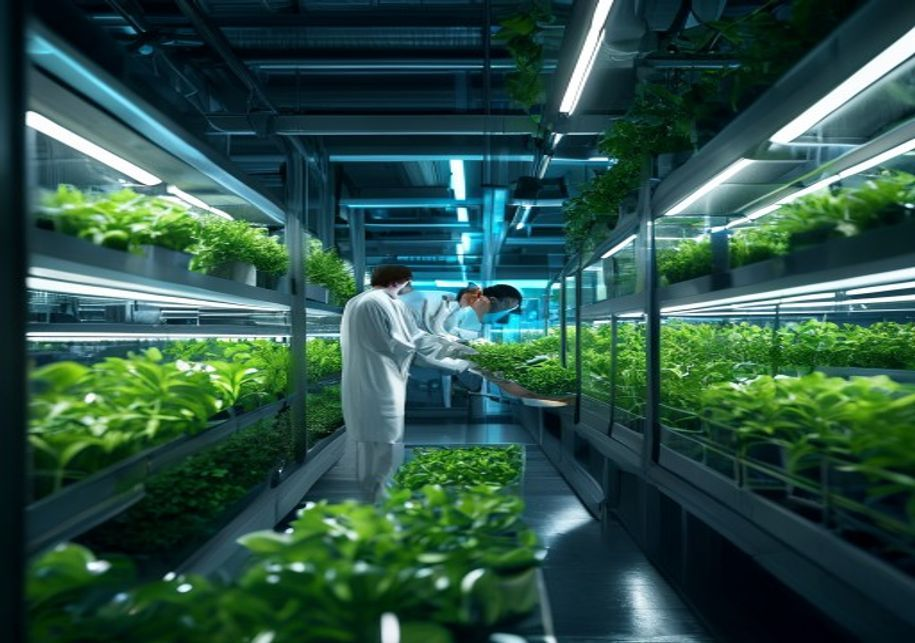
\includegraphics[width=58mm,height=45mm,keepaspectratio]{assets/image-6.png}
\end{minipage}
\vspace{3pt}\noindent\fcolorbox{BOLine}{BOLight}{\parbox{0.965\linewidth}{\small \textbf{So what:} \textbullet\ Validate assumptions with source backup.}}\vspace{4pt}
{\small {\small For traditional agribusinesses, alternative proteins and vertical farming represent both a threat and an opportunity. Companies that diversify into these adjacencies can capture new revenue streams and hedge against declining demand for conventional products. However, challenges remain, including high production costs, consumer acceptance, and regulatory hurdles. Strategic partnerships with technology startups and investments in R\&D are essential to navigate this transition successfully.}}
\vspace{4pt}{\textcolor{BOBlue}{\scriptsize\bfseries ANALYTIC CHECKLIST}}\par\begin{tabularx}{\linewidth}{p{42mm}Y}
Risk & Mitigation \\ 
Evidence quality & Validate sources \\ 
Adoption delay & Focus urgent buyers \\ 
\end{tabularx}

\clearpage
{\textcolor{BOBlue}{\scriptsize\bfseries CHAPTER 7}}\par\vspace{-1pt}
{\Large\sffamily\bfseries\color{BONavy} Carbon markets create new revenue streams but require verification standards}\par\vspace{4pt}
\begin{minipage}[t]{0.58\linewidth}
{\small Carbon farming, which involves agricultural practices that sequester carbon in soil and biomass, is emerging as a significant revenue opportunity for farmers. Practices such as cover cropping, reduced tillage, and agroforestry can sequester 0.5 to 2 tons of carbon per hectare per year. Voluntary carbon markets are growing rapidly, with prices for agricultural carbon credits ranging from \$15 to \$50 per ton, depending on quality and verification standards.}

{\small The potential for carbon markets to transform agricultural economics is substantial. A farmer adopting regenerative practices could earn \$30-\$100 per hectare annually from carbon credits, in addition to productivity gains from improved soil health. However, the market is fragmented, with multiple registries and methodologies creating confusion and inconsistency. Verification standards are critical to ensure that credits represent genuine, additional, and permanent carbon sequestration.}
\end{minipage}\hfill
\begin{minipage}[t]{0.36\linewidth}

\includegraphics[width=58mm,height=45mm,keepaspectratio]{assets/image-7.png}
\end{minipage}
\vspace{3pt}\noindent\fcolorbox{BOLine}{BOLight}{\parbox{0.965\linewidth}{\small \textbf{So what:} \textbullet\ Validate assumptions with source backup.}}\vspace{4pt}
{\small {\small To realize the full potential of carbon farming, industry stakeholders must collaborate to establish robust, science-based verification protocols. Agribusinesses can play a leading role by developing carbon measurement tools, offering carbon credit aggregation services, and integrating carbon revenue into their business models. Policymakers should support the development of standardized methodologies and provide incentives for adoption, such as tax credits or subsidies for carbon farming practices.}}
\vspace{4pt}{\textcolor{BOBlue}{\scriptsize\bfseries ANALYTIC CHECKLIST}}\par\begin{tabularx}{\linewidth}{p{42mm}Y}
Market signal & Structural demand \\ 
Capability & Scale and proof \\ 
Execution & Risks and actions \\ 
\end{tabularx}

\clearpage
{\textcolor{BOBlue}{\scriptsize\bfseries CHAPTER 8}}\par\vspace{-1pt}
{\Large\sffamily\bfseries\color{BONavy} Strategic priorities for the next 3-5 years require decisive action}\par\vspace{4pt}
\begin{minipage}[t]{0.58\linewidth}
{\small Based on the analysis, seven strategic priorities emerge for senior executives and policymakers. First, accelerate investment in digital and precision agriculture to boost productivity and resilience. Second, implement water and soil health programs to mitigate the most critical long-term risks. Third, diversify into alternative proteins and vertical farming to capture high-growth adjacencies. Fourth, engage with carbon markets to create new revenue streams and enhance sustainability credentials.}

{\small Fifth, adapt to regulatory shifts in Europe and trade tensions by diversifying supply chains and developing premium products. Sixth, bridge the digital divide to ensure inclusive growth and access to technology for smallholders. Seventh, build strategic partnerships across the value chain, including technology providers, research institutions, and governments, to drive innovation and scale solutions.}
\end{minipage}\hfill
\begin{minipage}[t]{0.36\linewidth}

\includegraphics[width=58mm,height=45mm,keepaspectratio]{assets/image-8.png}
\end{minipage}
\vspace{3pt}\noindent\fcolorbox{BOLine}{BOLight}{\parbox{0.965\linewidth}{\small \textbf{So what:} \textbullet\ Validate assumptions with source backup.}}\vspace{4pt}
{\small {\small These priorities require decisive action and significant investment, but the cost of inaction is far greater. Agribusinesses that lead in sustainability, technology adoption, and risk management will be best positioned to thrive in the coming decade. Policymakers must create enabling environments through supportive regulations, infrastructure investment, and public-private collaboration. The window for action is narrowing, but the opportunities for those who act now are immense.}}
\vspace{4pt}{\textcolor{BOBlue}{\scriptsize\bfseries ANALYTIC CHECKLIST}}\par\begin{tabularx}{\linewidth}{p{42mm}Y}
Use case & Priority logic \\ 
Near term & Clear proof path \\ 
Longer term & Monitor options \\ 
\end{tabularx}

\clearpage
{\textcolor{BOBlue}{\scriptsize\bfseries REFERENCE NOTE}}\par\vspace{-1pt}
{\small\color{BOMuted} This report was informed by public research and data from: Ipcc, Fao, Wri, Bloomberg, Marketsandmarkets, Grandviewresearch, Ecosystemmarketplace, Europa. Full source backup is archived in the backup folder.}

\end{document}
